%%%%%%%%%%%%%%%%%%%%%%%%%%%%%%%%%%%%%%%%%%%%%%%%%%%%%%%%%%%%%%%%%%%%%
%% This is a (brief) model paper using the achemso class
%% The document class accepts keyval options, which should include
%% the target journal and optionally the manuscript type. 
%%%%%%%%%%%%%%%%%%%%%%%%%%%%%%%%%%%%%%%%%%%%%%%%%%%%%%%%%%%%%%%%%%%%%
\documentclass[journal=jacsat,manuscript=article]{achemso}

%%%%%%%%%%%%%%%%%%%%%%%%%%%%%%%%%%%%%%%%%%%%%%%%%%%%%%%%%%%%%%%%%%%%%
%% Place any additional packages needed here.  Only include packages
%% which are essential, to avoid problems later. Do NOT use any
%% packages which require e-TeX (for example etoolbox): the e-TeX
%% extensions are not currently available on the ACS conversion
%% servers.
%%%%%%%%%%%%%%%%%%%%%%%%%%%%%%%%%%%%%%%%%%%%%%%%%%%%%%%%%%%%%%%%%%%%%
\usepackage[version=3]{mhchem} % Formula subscripts using \ce{}
\usepackage{siunitx}
\usepackage{graphicx}

%%%%%%%%%%%%%%%%%%%%%%%%%%%%%%%%%%%%%%%%%%%%%%%%%%%%%%%%%%%%%%%%%%%%%
%% If issues arise when submitting your manuscript, you may want to
%% un-comment the next line.  This provides information on the
%% version of every file you have used.
%%%%%%%%%%%%%%%%%%%%%%%%%%%%%%%%%%%%%%%%%%%%%%%%%%%%%%%%%%%%%%%%%%%%%
%%\listfiles

%%%%%%%%%%%%%%%%%%%%%%%%%%%%%%%%%%%%%%%%%%%%%%%%%%%%%%%%%%%%%%%%%%%%%
%% Place any additional macros here.  Please use \newcommand* where
%% possible, and avoid layout-changing macros (which are not used
%% when typesetting).
%%%%%%%%%%%%%%%%%%%%%%%%%%%%%%%%%%%%%%%%%%%%%%%%%%%%%%%%%%%%%%%%%%%%%
\newcommand*\mycommand[1]{\texttt{\emph{#1}}}

%%%%%%%%%%%%%%%%%%%%%%%%%%%%%%%%%%%%%%%%%%%%%%%%%%%%%%%%%%%%%%%%%%%%%
%% Meta-data block
%% ---------------
%% Each author should be given as a separate \author command.
%%
%% Corresponding authors should have an e-mail given after the author
%% name as an \email command. Phone and fax numbers can be given
%% using \phone and \fax, respectively; this information is optional.
%%
%% The affiliation of authors is given after the authors; each
%% \affiliation command applies to all preceding authors not already
%% assigned an affiliation.
%%
%% The affiliation takes an option argument for the short name.  This
%% will typically be something like "University of Somewhere".
%%
%% The \altaffiliation macro should be used for new address, etc.
%% On the other hand, \alsoaffiliation is used on a per author basis
%% when authors are associated with multiple institutions.
%%%%%%%%%%%%%%%%%%%%%%%%%%%%%%%%%%%%%%%%%%%%%%%%%%%%%%%%%%%%%%%%%%%%%
\author{Haruya Ishida}
\affiliation[Kyushu University]
{Department of Aeronautics and Astronautics, Kyushu University, Nishi-Ku, Motooka 744, Fukuoka 819-0395, Japan}
\author{Hideaki Teshima}
\affiliation[Kyushu University]
{Department of Aeronautics and Astronautics, Kyushu University, Nishi-Ku, Motooka 744, Fukuoka 819-0395, Japan}
\email{hteshima05@aero.kyushu-u.ac.jp}
\alsoaffiliation[I2CNER]
{International Institute for Carbon-Neutral Energy Research (WPI-I2CNER), Kyushu University, Nishi-Ku, Motooka 744, Fukuoka 819-0395, Japan}
\author{Koji Takahashi}
\affiliation[Kyushu University]
{Department of Aeronautics and Astronautics, Kyushu University, Nishi-Ku, Motooka 744, Fukuoka 819-0395, Japan}
\alsoaffiliation[I2CNER]
{International Institute for Carbon-Neutral Energy Research (WPI-I2CNER), Kyushu University, Nishi-Ku, Motooka 744, Fukuoka 819-0395, Japan}
\author{Vishwanath Ganesan}
\affiliation[UIUC MechSE]
{Department of Mechanical Science and Engineering, University of Illinois at Urbana-Champaign, Urbana, IL, USA}
\author{Nenad Miljkovic}
\affiliation[I2CNER]
{International Institute for Carbon-Neutral Energy Research (WPI-I2CNER), Kyushu University, Nishi-Ku, Motooka 744, Fukuoka 819-0395, Japan}
\alsoaffiliation[UIUC MechSE]
{Department of Mechanical Science and Engineering, University of Illinois at Urbana-Champaign, Urbana, IL, USA}
\alsoaffiliation[UIUC MRL]
{Materials Research Laboratory, University of Illinois at Urbana-Champaign, Urbana, IL, USA}
\alsoaffiliation[UIUC ECE]
{Department of Electrical and Computer Engineering, University of Illinois at Urbana-Champaign, Urbana, IL, USA}
\alsoaffiliation[iSEE]
{Institute for Sustainability, Energy and Environment (iSEE), University of Illinois at Urbana-Champaign, Urbana, IL, USA}
\alsoaffiliation[ARC]
{Air Conditioning and Refrigeration Center, University of Illinois at Urbana-Champaign, Urbana, IL, USA}

%%%%%%%%%%%%%%%%%%%%%%%%%%%%%%%%%%%%%%%%%%%%%%%%%%%%%%%%%%%%%%%%%%%%%
%% The document title should be given as usual. Some journals require
%% a running title from the author: this should be supplied as an
%% optional argument to \title.
%%%%%%%%%%%%%%%%%%%%%%%%%%%%%%%%%%%%%%%%%%%%%%%%%%%%%%%%%%%%%%%%%%%%%
\title[title]
  {Hydrophobic Surfaces Are Not Slippery: Insights from Nanoscale Slip Length Mapping}

%%%%%%%%%%%%%%%%%%%%%%%%%%%%%%%%%%%%%%%%%%%%%%%%%%%%%%%%%%%%%%%%%%%%%
%% Some journals require a list of abbreviations or keywords to be
%% supplied. These should be set up here, and will be printed after
%% the title and author information, if needed.
%%%%%%%%%%%%%%%%%%%%%%%%%%%%%%%%%%%%%%%%%%%%%%%%%%%%%%%%%%%%%%%%%%%%%
\abbreviations{IR,NMR,UV}
\keywords{American Chemical Society, \LaTeX}

%%%%%%%%%%%%%%%%%%%%%%%%%%%%%%%%%%%%%%%%%%%%%%%%%%%%%%%%%%%%%%%%%%%%%
%% The manuscript does not need to include \maketitle, which is
%% executed automatically.
%%%%%%%%%%%%%%%%%%%%%%%%%%%%%%%%%%%%%%%%%%%%%%%%%%%%%%%%%%%%%%%%%%%%%
\begin{document}

%%%%%%%%%%%%%%%%%%%%%%%%%%%%%%%%%%%%%%%%%%%%%%%%%%%%%%%%%%%%%%%%%%%%%
%% The "tocentry" environment can be used to create an entry for the
%% graphical table of contents. It is given here as some journals
%% require that it is printed as part of the abstract page. It will
%% be automatically moved as appropriate.
%%%%%%%%%%%%%%%%%%%%%%%%%%%%%%%%%%%%%%%%%%%%%%%%%%%%%%%%%%%%%%%%%%%%%
\begin{tocentry}

Some journals require a graphical entry for the Table of Contents.
This should be laid out ``print ready'' so that the sizing of the
text is correct.

Inside the \texttt{tocentry} environment, the font used is Helvetica
8\,pt, as required by \emph{Journal of the American Chemical
Society}.

The surrounding frame is 9\,cm by 3.5\,cm, which is the maximum
permitted for  \emph{Journal of the American Chemical Society}
graphical table of content entries. The box will not resize if the
content is too big: instead it will overflow the edge of the box.

This box and the associated title will always be printed on a
separate page at the end of the document.

\end{tocentry}

%%%%%%%%%%%%%%%%%%%%%%%%%%%%%%%%%%%%%%%%%%%%%%%%%%%%%%%%%%%%%%%%%%%%%
%% The abstract environment will automatically gobble the contents
%% if an abstract is not used by the target journal.
%%%%%%%%%%%%%%%%%%%%%%%%%%%%%%%%%%%%%%%%%%%%%%%%%%%%%%%%%%%%%%%%%%%%%
\begin{abstract}
  While slip at solid-liquid interfaces has attracted broad interest, slip lengths reported in experiments—especially on hydrophobic surfaces (i.e. contact angles \(> \SI{90}{degree}\))—vary widely due to surface topographical and chemical heterogeneity, hindering quantitative understanding of the true slip length. Using highly sensitive frequency-modulation atomic force microscopy, we achieved simultaneous nanoscale mapping of slip length and surface topography, with a 159-fold improvement in slip length detection sensitivity. True slip lengths measured on flat regions of various substrates were found to be almost zero, following a scaling rule predicted by molecular dynamics simulations. As the only exception, a large slip length of \(43.2 \pm \SI{5.8}{\nano\metre}\) was measured on graphite in deionized water, but it vanished upon immersion in electrolyte solutions. This unique behavior was rationalized by graphite's atomic-scale smoothness, chemical homogeneity, and ion adsorption. Our method experimentally advances a unified picture of fluid slip.
\end{abstract}

%%%%%%%%%%%%%%%%%%%%%%%%%%%%%%%%%%%%%%%%%%%%%%%%%%%%%%%%%%%%%%%%%%%%%
%% Start the main part of the manuscript here.
%%%%%%%%%%%%%%%%%%%%%%%%%%%%%%%%%%%%%%%%%%%%%%%%%%%%%%%%%%%%%%%%%%%%%
\section{main}

The no-slip boundary condition, which assumes that the fluid velocity at a solid wall is zero, has long been regarded as an implicit premise in fluid mechanics. However, recent experiments have reported the occurrence of boundary slip, where fluids slip along solid surfaces with a finite velocity [1-7]. Slip is quantified by the slip length \(b\), defined in terms of the slip flow velocity \(v_{s}\) and the shear rate \(\partial v / \partial z \), as follows [8]: 

\begin{equation}
  v_s = b \left( \frac{\partial v}{\partial z} \right)_{z=0}. \label{eqn:definition of slip length}
\end{equation}

Solid-liquid friction is drastically reduced when slip occurs. For instance, the flow rate of water through carbon nanotubes [9] and hydrophobic fluorous nanochannels [10] has been reported to exceed continuum predictions by orders of magnitude. Such enhancements are decisive factors for the performance of nanofluidic devices, in which interfacial effects are dominant. Thus, efficient molecular transport realized by the control of slip is highly desired for breakthroughs in desalination [10], lab-on-a-chip technologies [11], osmotic power generators [12,13], and on-chip cooling [14,15].

Previous studies have suggested that solid-liquid interfacial properties such as wettability [16], surface roughness [17], surface charge [18], surface free energy distribution [19], and surface nanobubbles [20] strongly influence the slip length. However, despite extensive efforts, their quantitative relationships remain unclear. In particular, compared with hydrophilic surfaces (i.e., contact angles \(< \SI{90}{degree}\)), there is no clear consensus on slip lengths for hydrophobic surfaces (i.e., contact angles \(> \SI{90}{degree}\)). A scaling law relating the slip length \(b\) to the intrinsic contact angle \(\theta\) is derived as follows [16]:

\begin{equation}
  b = \frac{C}{(1 + \cos \theta)^{2}}. \label{eqn:slip length scaling}
\end{equation}

where \(C\) is a proportionality constant. Slip lengths obtained from molecular dynamics (MD) simulations are well fit by (Eq.~\ref{eqn:slip length scaling}) with \(C = 0.41\), indicating almost no slip even at intrinsic contact angles of \SI{120}{\degree}, which is the near maximum achievable on a topographically smooth flat surface [21]. In contrast, others compiled 11 experimental studies and reported that \(C = 6.0\), corresponding to slip lengths of several tens of nanometers at contact angles around \SI{90}{\degree} [22]. Moreover, other experimental studies beyond the compilation in Ref. [22] have shown notable deviations from this trend; on hydrophobic surfaces, both nearly no slip [23,24] and a slip length as large as \SI{1}{\micro\metre} [25] have been detected. 

This discrepancy between experiments and MD analyses is likely due to a complex interplay of multiple factors, not only measurement artifacts [26]  but also nanoscale interfacial effects, such as reduced friction caused by nanobubbles [20] and apparent slip lengths arising from nanoscopic surface roughness [27]. No existing technique can measure slip lengths while explicitly accounting for these interfacial effects. As a result, the measured (apparent) slip lengths can deviate from the intrinsic values, making experimental investigations of true slip highly challenging. In other words, we still cannot answer the simple yet long-standing question: “Does water slip on hydrophobic surfaces?”

To date, atomic force microscopy (AFM) provides the highest lateral spatial resolution for slip length measurements [4-7]. However, in practice, the lateral resolution is typically limited to approximately \SI{10}{\micro\metre} because of limited detection sensitivity, which is still insufficient for accurate slip length measurements.

In this study, we dramatically improve the spatial resolution of slip length measurements by employing highly sensitive frequency-modulation (FM) AFM. In AFM-based slip measurements, the viscous drag force \(F_h\) acting on the sphere of an AFM probe tip near a planar substrate is given by:

\begin{equation}
F_h=-\gamma_{\text{tip}} \dot{h}=-\frac{6\pi\eta R^2 \dot{h}}{h} f^* (b_t,b_s). \label{eqn:hydrodynamic force}
\end{equation}

where \(\gamma_{\text{tip}}\) is the viscous damping coefficient acting on the probe tip,  \(\eta\) is the viscosity of the surrounding medium, \(R\) is the radius of curvature of the probe tip, \(h\) is the probe-substrate distance, \(b_t\) and \(b_s\) are the slip lengths at the probe tip and substrate surfaces, respectively, and \(f^*\) is a correction factor representing the reduction of viscous drag due to slip [5]. In conventional contact-mode AFM, \(F_h\) is determined from the static deflection of the cantilever and the viscous drag scales with \(R^2\) as shown in Eq.~\ref{eqn:hydrodynamic force}.  Consequently, when the probe radius is reduced, the detection sensitivity rapidly decreases. Although the smallest probe radius reported to date is \(R = \SI{1.9}{\micro\metre}\) [6], probe tips with radii of approximately \(\SI{10}{\micro\metre}\) [7] are typically used, and further miniaturization remains challenging.

To overcome this limitation, we employ FM-AFM [28], in which the cantilever is continuously oscillated at its resonance frequency. In this mode, the energy dissipated by viscous drag is quantified as the damping coefficient \(\gamma\). Because the resonance amplifies the viscous drag, the sensitivity to it is significantly enhanced, thereby compensating for the signal-to-noise degradation proportional to \(R^2\). Then, \(\gamma_{\text{tip}}\) can be obtained from the oscillation amplitudes \(A_{\text{bulk}}\) and \(A(h)\) (see Supplemental Material, Sec. I, for details [44]):

\begin{equation}
\gamma_{\text{tip}} (h,b_t,b_s)=\gamma_{\text{bulk}} \left(\frac{A_{\text{bulk}}}{A(h)} -1\right). \label{eqn:damping coefficient amplitude}
\end{equation}

where the subscript "bulk" denotes the value at sufficiently large \(h\). In conventional FM-AFM, the oscillation amplitude is kept constant (\(A(h) = A_{\text{bulk}}\) = const.) by an automatic gain control (AGC) circuit. However, in our method, the AGC is turned off and instead the drive power is kept constant, allowing the amplitude reduction \(A(h)\) to directly reflect the magnitude of the damping coefficient \(\gamma_{\text{tip}}\). This offers the advantage that the reliability of slip length measurements is not limited by AGC performance. Extracting the coefficient of \(\dot{h}\) from Eq.~\ref{eqn:hydrodynamic force}, the damping coefficient can be expressed as

\begin{equation}
\gamma_{\text{tip}} (h,b_t,b_s)=\frac{6\pi\eta R^2}{h} f^* (b_t,b_s). \label{eqn:damping coefficient slip}
\end{equation}

Slip length \(b_s\) is then obtained by fitting Eq.~\ref{eqn:damping coefficient slip} to a damping-coefficient-tip-sample distance curve with \(b_s\) as the fitting parameter. We note that the slip length of the probe material, \(b_t\), needs to be pre-calibrated using a substrate made of the same material (\(b_t=b_s\)). This method enhances slip length sensitivity by 159-fold relative to normal contact-mode AFM (see Supplemental Material, Sec. II, for details [44]). Consequently, this allows us to measure the slip length using a probe with a much smaller sphere. 

\begin{figure}[h]
  \centering
  \includegraphics[width=1.0\linewidth]{figs/schematics_of_measurement.png}
  \caption{(a) Total damping coefficient \(\gamma_{\text{total}}\) as a function of probe tip-sample distance \(h\) measured at an HOPG-deionized water interface. Blue dots indicate the experimental data. The black dashed and red solid lines represent theoretical curves for a no-slip boundary condition (\(b_s = 0\)) and a fitted slip length (\(b_s = \SI{43.2}{\nano\metre}\)), respectively. (b, c) SEM images of the probe with a diamond-like carbon spherical tip. (d) Schematic illustration of the simultaneous mapping of slip length and topography using FM-AFM. The color bar indicates the total damping coefficient.}
  \label{fgr:schematics_of_measurement}
\end{figure}

In (Figure~\ref{fgr:schematics_of_measurement}(a)), we show a representative damping-coefficient-tip-sample distance curve obtained at an interface between deionized water (Milli-Q, Millipore, USA) and highly oriented pyrolytic graphite (HOPG, SPI-1 grade; Alliance Biosystems, Japan). This measurement was performed with a colloidal probe having a \(\SI{300}{\nano\metre}\) radius of curvature (Biosphere B300-NCH, Nanotools), which is about one-thirtieth of the radius typically used in past studies. SEM images of the probe are shown in (Figures~\ref{fgr:schematics_of_measurement}(b) and (c)). The resonance frequency \(f_0\) and quality factor \(Q_{\text{bulk}}\) of the cantilever in water, as well as its spring constant \(k\), were identified by thermal-noise analysis [29,30]. For the measurement in (Figure~\ref{fgr:schematics_of_measurement}(a)), we obtained \(f_0 = \SI{145.8}{\kilo\hertz}\), \(Q_{\text{bulk}} = 8.2\), and \(k = \SI{22}{\newton\per\metre}\). The measured total damping \(\gamma_{\text{total}}=\gamma_{\text{tip}}+\gamma_{\text{bulk}}\) was consistently smaller than the theoretical curve for a no-slip assumption (\(b_s = \SI{0}{\nano\metre}\)), whereas it was well fitted by the curve with \(b_s = \SI{43.2}{\nano\metre}\), demonstrating the utility of our new method.

Next, we extended this method to perform simultaneous nanoscale mapping of slip length and surface topography. A schematic of the measurement principle and representative three-dimensional maps of the damping coefficient are shown in (Figure~\ref{fgr:schematics_of_measurement}(d)). Measurements were performed using the ZXY scan mode of an SPM-8100FM (Shimadzu Corp., Japan) equipped with a custom-built photothermal excitation system and a closed-loop feedback scanner. At each \((x, y)\) pixel on the sample plane, the probe was scanned in the \(z\)-direction while recording the cantilever deflection, amplitude, and frequency-shift. The topography was reconstructed from the deflection, whereas the slip length was determined from the damping coefficient using Eq.~\ref{eqn:damping coefficient slip}. 

Slip length mapping was first carried out on HOPG and on a hydrophilic-hydrophobic composite substrate (oxygen plasma treated silica-1H,1H,2H,2H-perfluorooctanephosphonic acid, FOPA; the fabrication procedures are in Supplemental Material, Sec. III-A [44]). The contact angles of deionized-water droplets, measured separately on the hydrophilic and hydrophobic surfaces, were \(\SI{28}{\degree}\) and \(\SI{105}{\degree}\), respectively. The composite substrate enabled us to test artificially fabricated patterns, whereas HOPG, with its atomically flat terraces and step structures [31], served as a natural reference surface for verifying nanoscale spatial resolution. Prior to measurement, the HOPG surface was freshly cleaved with Scotch tape to expose a clean surface. Before each measurement, the cantilever was hydrophilized by atmospheric plasma treatment. In all measurements, the cantilever was controlled to oscillate with an amplitude of \(\SI{2}{\nano\metre}\). We calibrated the slip length of the probe tip by measuring a symmetric system (\(b_t = b_s\)) using an atmospheric-plasma-treated diamond-like carbon (DLC) substrate, yielding a slip length of \(b_t = b_s = 0.0 \pm \SI{1.2}{\nano\metre}\). 

\begin{figure}[h]
  \centering
  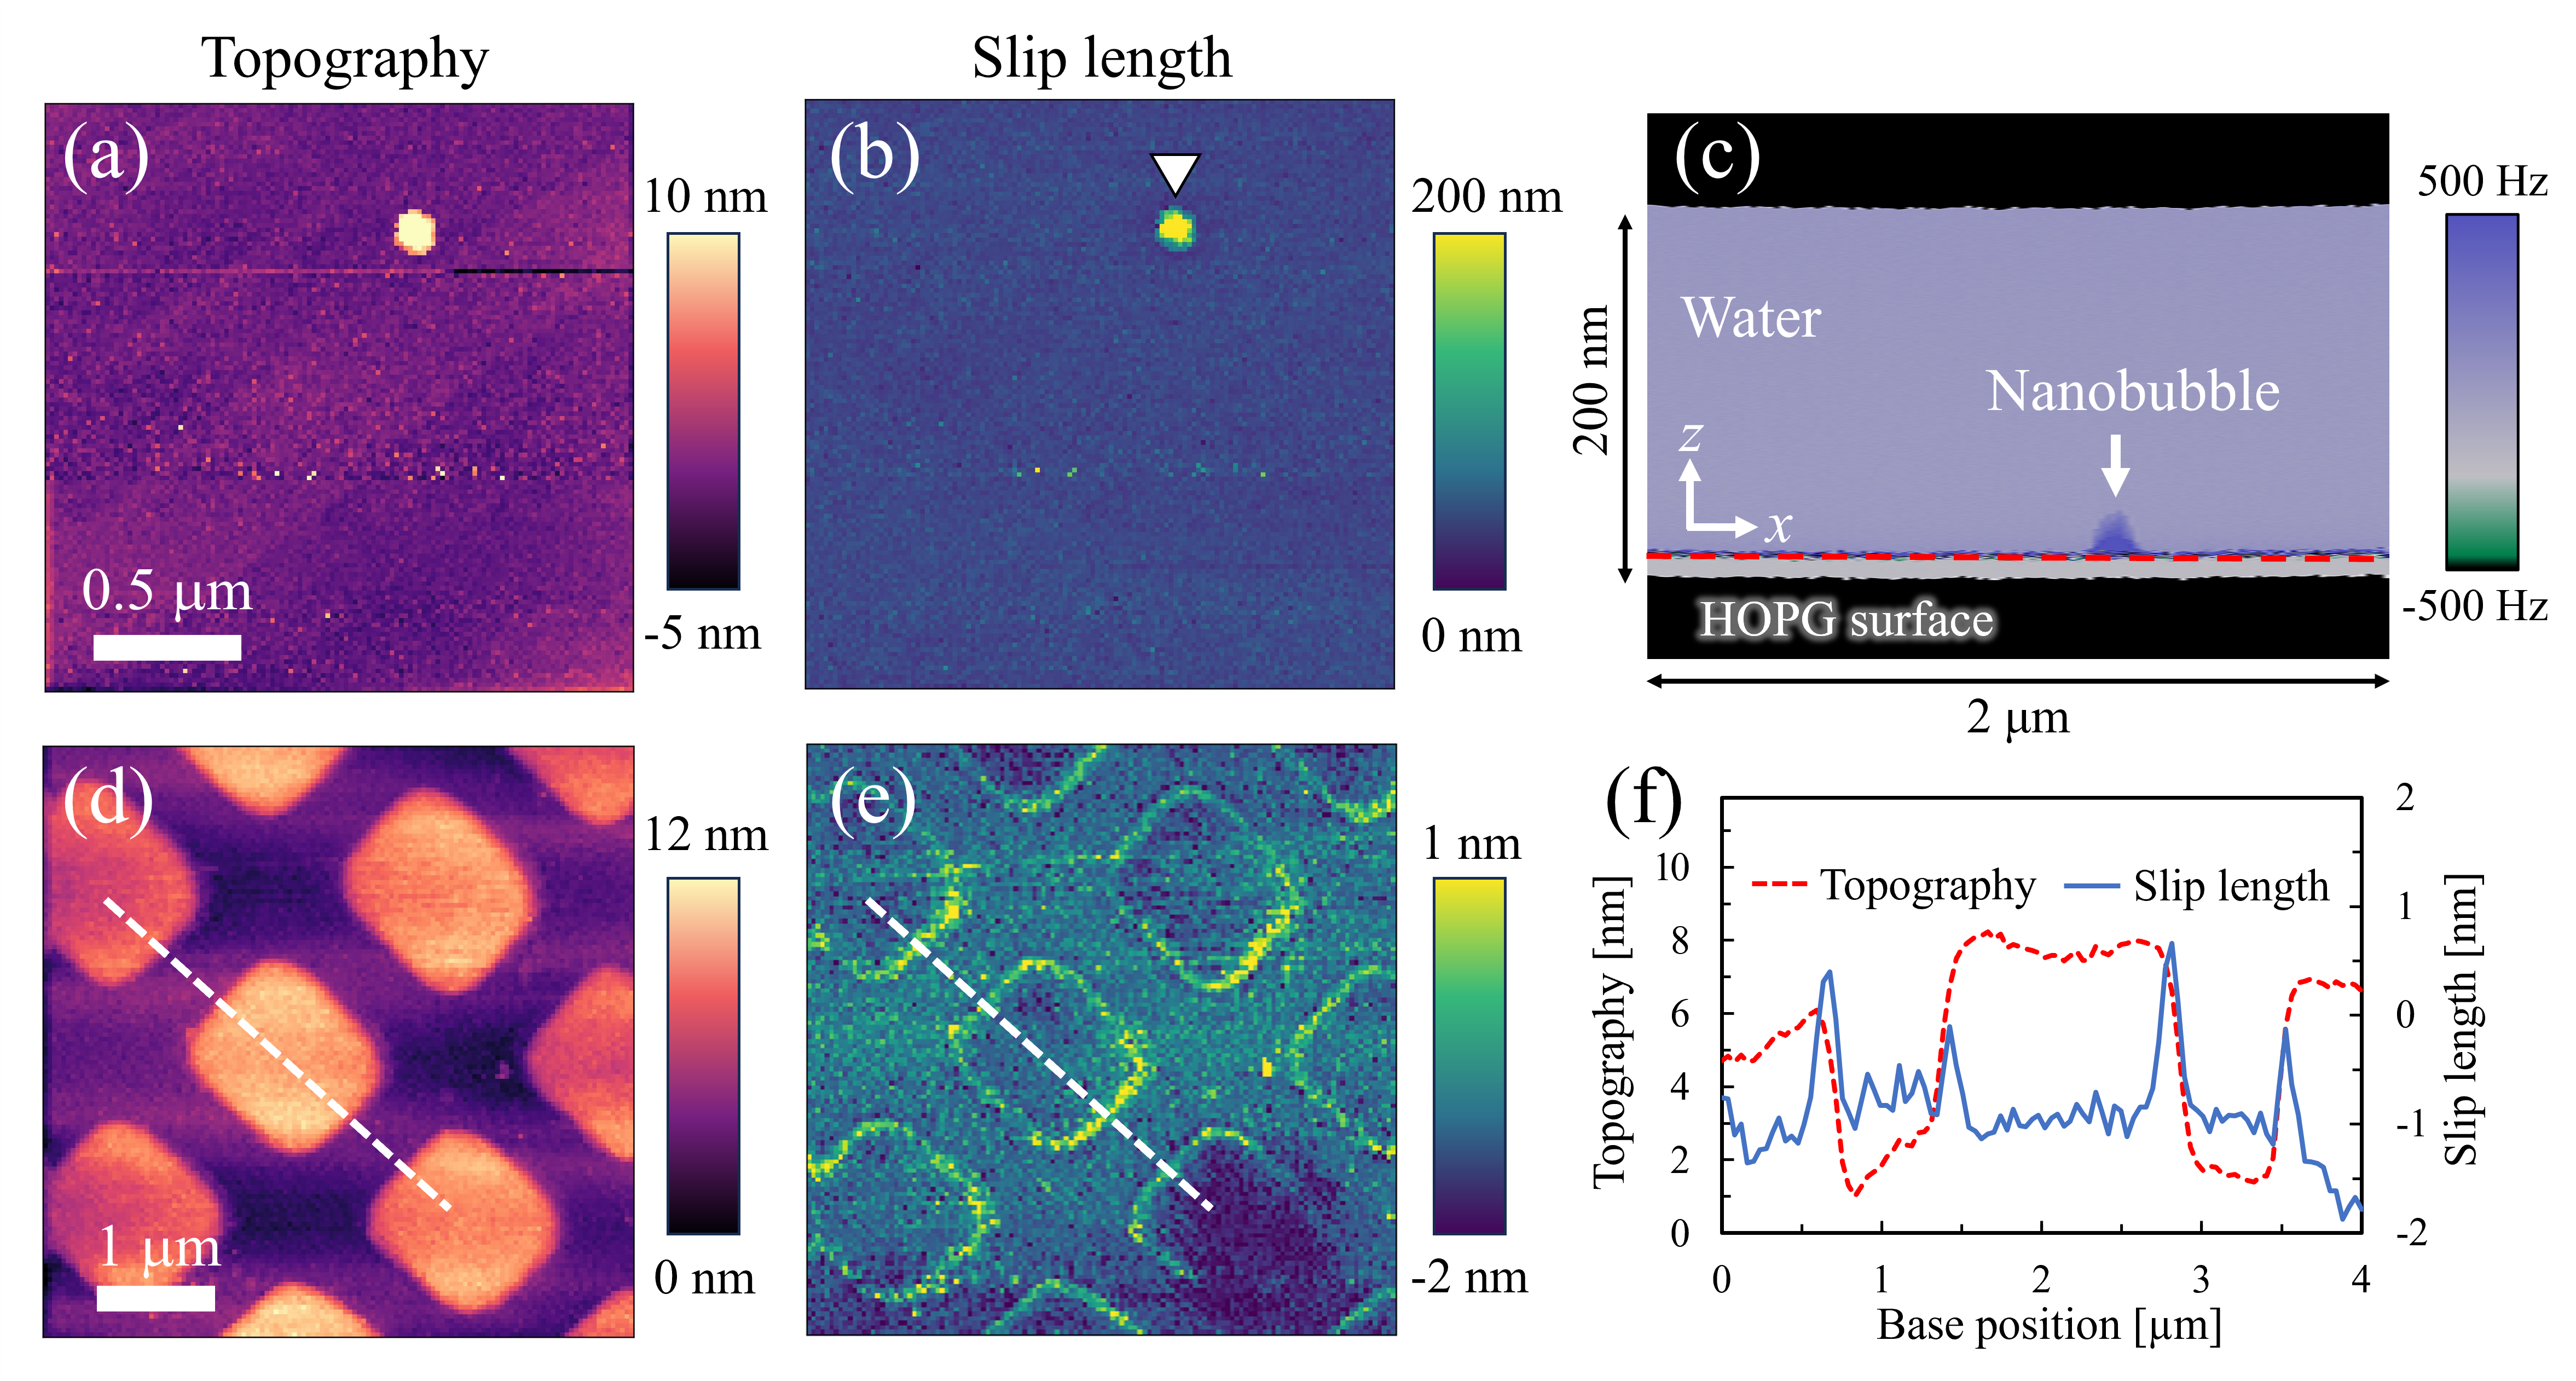
\includegraphics[width=1.0\linewidth]{figs/mapping_results.png}
  \caption{(a) Surface topography and (b) slip length maps on the HOPG surface. The average slip length was 43.2 ± \SI{5.8}{\nano\meter}. (c) Z-X frequency-shift image along the location where a nanobubble was detected, as indicated by the white triangle in (b). The red dashed line corresponds to the HOPG surface. (d) Surface topography and (e) slip length on the FOPA-silica composite surface. The FOPA patches are \(\SI{1}{\micro\meter} \times \SI{1}{\micro\meter}\) in lateral size and \SI{5}{\nano\meter} in height. (f) Cross-sectional profiles of the topography and slip length along the white dashed lines indicated in (d) and (e).}
  \label{fgr:mapping_results}
\end{figure}

(Figure~\ref{fgr:mapping_results}) clearly demonstrates that the present method enables simultaneous nanoscale visualization of topography and slip length. (Figure~\ref{fgr:mapping_results}(a)) not only reveals the presence of fine terrace structures \(\sim\SI{100}{\nano\metre}\) in width, but also resolves single graphene steps with heights of \(\SI{0.34}{\nano\metre}\) [32]. On the flat area of the HOPG surface, a large slip length of \(43.2 \pm \SI{5.8}{\nano\metre}\) was obtained (Figure~\ref{fgr:mapping_results}(b)). Remarkably, a spherical region with significantly reduced slip length compared with the surrounding area appeared, as indicated by the white triangle. In the Z-X frequency-shift cross section (Figure~\ref{fgr:mapping_results}(c)) taken across this region, we detected a feature that clearly protrudes from the HOPG surface and exhibits an enhanced frequency shift. We conclude that this is an incidentally formed nanobubble. Because a positive frequency shift corresponds to repulsive forces, the observed enhancement indicates that the hydrophilized probe experienced repulsion when pushing this region, a characteristic response to nanobubbles [33,34]. The object exhibited a contact radius of \(\SI{72.3}{\nano\metre}\), a height of \(\SI{22.2}{\nano\metre}\), and a contact angle of \(\SI{146}{\degree}\). These are in good agreement with values typically reported in previous studies [35,36], verifying that the observed structure is indeed a surface nanobubble. 

Because topography is reconstructed based on the position at which the probe mechanically contacts the substrate, the nanobubble did not appear in the height image. The slip reduction is because the calculated slip length was defined with respect to the solid surface; in reality, the slip length at the liquid-gas interface is expected to be much larger. Thus, our method can detect nanobubbles and even assess their local slip properties. 

In (Figure~\ref{fgr:mapping_results}(d)),  FOPA patches, only \(\SI{5}{\nano\metre}\) in height, are clearly visualized, and their boundaries exhibit a distinct increase in slip length (Figure~\ref{fgr:mapping_results}(e)) because the gap beneath the step facilitates fluid flow when the probe contacts the substrate [37]. This increase was also confirmed in the cross-sectional profiles of the topography and slip length (Figure~\ref{fgr:mapping_results}(f)), which clearly show a rise in slip length at the edges of the patch. Therefore, the large slip lengths observed near the edges represent apparent rather than true slip lengths, indicating that our measurement system can faithfully resolve local interfacial geometry. On the flat silica and FOPA regions, slip lengths of \(-0.7 \pm \SI{0.6}{\nano\metre}\) and \(-0.9 \pm \SI{0.6}{\nano\metre}\), respectively, were obtained, both indicating a no-slip boundary condition, which contradicts many experimental studies reporting larger slip lengths on hydrophobic surfaces [22,25]. Thus, we hypothesize that the previously reported large slip lengths may have resulted from the effects of surface structures or nanobubbles, and therefore represent apparent slip lengths rather than true ones.

Next, we systematically measured slip lengths on a variety of solid surfaces with contact angles ranging from \(\SI{3}{\degree}\) to \(\SI{111}{\degree}\). The substrates used were silica, DLC, muscovite mica, HOPG, Octadecyltrichlorosilane (OTS), FOPA, 1H,1H,2H,2H-perfluorodecyltriethoxysilane (FDTS), and Teflon. DLC, OTS, FOPA, and FDTS were coated on flat Si substrates. Among the flat surfaces, Teflon exhibits one of the largest intrinsic contact angles [38,39]. The preparation of the Teflon substrate is described in the Supplemental Material, Sec. III-B [44].

\begin{figure}[h]
  \centering
  \includegraphics[width=0.6\linewidth]{figs/scaling_result.png}
  \caption{Systematic comparison of slip lengths on nanoscopically flat substrates with contact angles ranging from \SI{3}{\degree} to \SI{111}{\degree}. The error bar represents the standard deviation. The blue solid line represents the theoretical scaling law of Eq. (2) with \(C = 6.0\), and the red dashed line corresponds to \(C = 0.41\). The gray region represents contact angles that cannot be realized on real flat surfaces. The slip length maps obtained on all the surfaces are shown in Fig. S1 [44].}
  \label{fgr:scaling_result}
\end{figure}

(Figure~\ref{fgr:scaling_result}) presents the measured slip lengths on flat substrates. Interestingly, on all surfaces except HOPG, the slip lengths were almost zero, in good agreement with the scaling in Eq.~\ref{eqn:slip length scaling} when using the previously reported MD-based value \(C = 0.41\) [16] (red dashed line), rather than the experimental value \(C = 6.0\) [22] (blue solid line). This supports our interpretation that earlier experimental studies may have overestimated slip lengths due to the influence of nanoscale surface features. Even on the most hydrophobic sample (Teflon), the slip length was only \(0.8 \pm \SI{0.8}{\nano\metre}\), clearly indicating that the relation "hydrophobic surfaces exhibit large slip" does not hold.

In contrast, only HOPG (contact angle \(\SI{59.0}{\degree}\)) exhibited a markedly large slip length of \(43.2 \pm \SI{5.8}{\nano\metre}\), inconsistent with the scaling law. However, previous MD studies have reported that the atomic-scale smoothness of graphite drastically reduces friction, leading to the slip length on the order of \(\SI{50}{\nano\metre}\) [40,41]. Although mica also has atomically smooth surface, unlike graphite, which is composed solely of carbon atoms, its surface consists of four elements (K, Si, Al, and O). Such atomic-scale chemical heterogeneity leads to a more strongly corrugated interfacial energy landscape, as predicted by ab initio MD [19], resulting in an extremely small slip length. Therefore, our experimental results are in good agreement with past simulations. 

Interestingly, the slip length on HOPG decreased to \(-0.1 \pm \SI{0.7}{\nano\metre}\) when measured in a \(\SI{10}{\milli\mole\per\litre}\) KCl solution, indicating a no-slip boundary condition. This is because of surface charge. A recent MD study reported that even a slight charge on graphene surfaces (\(\sim\SI{20}{\milli\volt}\)) reduces the slip length from \(\SI{45}{\nano\metre}\) to \(\SI{2}{\nano\metre}\) in an electrolyte solution [18]. One major mechanism is that K\(^+\) ions selectively adsorb onto the charged graphene surface and, through their structured hydration shells, strongly pin water molecules to the surface [42]. Because actual graphene surfaces typically have a surface potential of \(\sim\SI{20}{\milli\volt}\) [43], adding electrolyte is expected to significantly suppress slip. A similar reduction was observed in a \(\SI{10}{\milli\mole\per\litre}\) NaCl solution (not shown in (Figure~\ref{fgr:scaling_result}), see Table S1 in Supplemental Material [44]). Paradoxically, these results suggest that controlling surface charge may offer a route to enhancing slip on graphite/graphene and potentially achieving appreciable slip on other surfaces, which we will investigate in future work.

In conclusion, we developed an experimental method for slip length measurement using FM-AFM and achieved a 159-fold improvement in slip length detection sensitivity. This enabled, for the first time, simultaneous nanoscale mapping of slip length and surface topography, allowing us to quantify the true slip length by excluding the influence of surface heterogeneities such as surface roughness and nanobubbles. A systematic investigation has resolved the long-standing discrepancy between experiments and MD simulations, leading to the conclusion that hydrophobic surfaces are not slippery. A large slip length in deionized water was observed only on the HOPG surface with mild wettability. This value became negligibly small when conducted in electrolyte solutions, in agreement with past MD analysis. This result demonstrates that slip length on flat surfaces depends more strongly on the crystalline structure than on wettability, highlighting the singular nature of graphite. Our method substantially improves the accuracy of slip length measurements and provides, to the best of our knowledge, the only experimental technique capable of quantitatively evaluating true slip and correlating it with nanoscale surface characteristics. This breakthrough not only bridges the long-standing gap between experiments and MD simulations, but also opens a new avenue for experimentally exploring how slip length is affected by factors that are difficult to reproduce in MD, such as electric double layers, nanobubbles, and hydrogels. 

\section{Results and discussion}

\subsection{Outline}

The document layout should follow the style of the journal concerned.
Where appropriate, sections and subsections should be added in the
normal way. If the class options are set correctly, warnings will be
given if these should not be present.

\subsection{References}

The class makes various changes to the way that references are
handled.  The class loads \textsf{natbib}, and also the
appropriate bibliography style.  References can be made using
the normal method; the citation should be placed before any
punctuation, as the class will move it if using a superscript
citation style
\cite{Mena2000,Abernethy2003,Friedman-Hill2003,EuropeanCommission2008}.
The use of \textsf{natbib} allows the use of the various citation
commands of that package: \citeauthor{Abernethy2003} have shown
something, in \citeyear{Cotton1999}, or as given by
Ref.~\citenum{Mena2000}.  Long lists of authors will be
automatically truncated in most article formats, but not in
supplementary information or reviews \cite{Pople2003}. If you
encounter problems with the citation macros, please check that
your copy of \textsf{natbib} is up to date. The demonstration
database file \texttt{achemso-demo.bib} shows how to complete
entries correctly. Notice that ``\latin{et al.}'' is auto-formatted
using the \texttt{\textbackslash latin} command.

Multiple citations to be combined into a list can be given as
a single citation.  This uses the \textsf{mciteplus} package
\cite{Johnson1972,*Arduengo1992,*Eisenstein2005,*Arduengo1994}.
Citations other than the first of the list should be indicated
with a star. If the \textsf{mciteplus} package is not installed,
the standard bibliography tools will still work but starred
references will be ignored. Individual references can be referred
to using \texttt{\textbackslash mciteSubRef}:
``ref.~\mciteSubRef{Eisenstein2005}''.

The class also handles notes to be added to the bibliography.  These
should be given in place in the document \bibnote{This is a note.
The text will be moved the the references section.  The title of the
section will change to ``Notes and References''.}.  As with
citations, the text should be placed before punctuation.  A note is
also generated if a citation has an optional note.  This assumes that
the whole work has already been cited: odd numbering will result if
this is not the case \cite[p.~1]{Cotton1999}.

\subsection{Floats}

New float types are automatically set up by the class file.  The
means graphics are included as follows (Scheme~\ref{sch:example}).  As
illustrated, the float is ``here'' if possible.
\begin{scheme}
  Your scheme graphic would go here: \texttt{.eps} format\\
  for \LaTeX\, or \texttt{.pdf} (or \texttt{.png}) for pdf\LaTeX\\
  \textsc{ChemDraw} files are best saved as \texttt{.eps} files:\\
  these can be scaled without loss of quality, and can be\\
  converted to \texttt{.pdf} files easily using \texttt{eps2pdf}.\\
  %\includegraphics{graphic}
  \caption{An example scheme}
  \label{sch:example}
\end{scheme}

\begin{figure}
  As well as the standard float types \texttt{table}\\
  and \texttt{figure}, the class also recognises\\
  \texttt{scheme}, \texttt{chart} and \texttt{graph}.
  \caption{An example figure}
  \label{fgr:example}
\end{figure}

Charts, figures and schemes do not necessarily have to be labelled or
captioned.  However, tables should always have a title. It is
possible to include a number and label for a graphic without any
title, using an empty argument to the \texttt{\textbackslash caption}
macro.

The use of the different floating environments is not required, but
it is intended to make document preparation easier for authors. In
general, you should place your graphics where they make logical
sense; the production process will move them if needed.

\subsection{Math(s)}

The \textsf{achemso} class does not load any particular additional
support for mathematics.  If packages such as \textsf{amsmath} are
required, they should be loaded in the preamble.  However,
the basic \LaTeX\ math(s) input should work correctly without
this.  Some inline material \( y = mx + c \) or $ 1 + 1 = 2 $
followed by some display. \[ A = \pi r^2 \]

It is possible to label equations in the usual way (Eq.~\ref{eqn:example}).
\begin{equation}
  \frac{\mathrm{d}}{\mathrm{d}x} \, r^2 = 2r \label{eqn:example}
\end{equation}
This can also be used to have equations containing graphical
content. To align the equation number with the middle of the graphic,
rather than the bottom, a minipage may be used.
\begin{equation}
  \begin{minipage}[c]{0.80\linewidth}
    \centering
    As illustrated here, the width of \\
    the minipage needs to allow some  \\
    space for the number to fit in to.
    %\includegraphics{graphic}
  \end{minipage}
  \label{eqn:graphic}
\end{equation}

\section{Experimental}

The usual experimental details should appear here.  This could
include a table, which can be referenced as Table~\ref{tbl:example}.
Notice that the caption is positioned at the top of the table.
\begin{table}
  \caption{An example table}
  \label{tbl:example}
  \begin{tabular}{ll}
    \hline
    Header one  & Header two  \\
    \hline
    Entry one   & Entry two   \\
    Entry three & Entry four  \\
    Entry five  & Entry five  \\
    Entry seven & Entry eight \\
    \hline
  \end{tabular}
\end{table}

Adding notes to tables can be complicated.  Perhaps the easiest
method is to generate these using the basic
\texttt{\textbackslash textsuperscript} and
\texttt{\textbackslash emph} macros, as illustrated (Table~\ref{tbl:notes}).
\begin{table}
  \caption{A table with notes}
  \label{tbl:notes}
  \begin{tabular}{ll}
    \hline
    Header one                            & Header two \\
    \hline
    Entry one\textsuperscript{\emph{a}}   & Entry two  \\
    Entry three\textsuperscript{\emph{b}} & Entry four \\
    \hline
  \end{tabular}

  \textsuperscript{\emph{a}} Some text;
  \textsuperscript{\emph{b}} Some more text.
\end{table}

The example file also loads the optional \textsf{mhchem} package, so
that formulas are easy to input: \texttt{\textbackslash ce\{H2SO4\}}
gives \ce{H2SO4}.  See the use in the bibliography file (when using
titles in the references section).

The use of new commands should be limited to simple things which will
not interfere with the production process.  For example,
\texttt{\textbackslash mycommand} has been defined in this example,
to give italic, mono-spaced text: \mycommand{some text}.

\section{Extra information when writing JACS Communications}

When producing communications for \emph{J.~Am.\ Chem.\ Soc.}, the
class will automatically lay the text out in the style of the
journal. This gives a guide to the length of text that can be
accommodated in such a publication. There are some points to bear in
mind when preparing a JACS Communication in this way.  The layout
produced here is a \emph{model} for the published result, and the
outcome should be taken as a \emph{guide} to the final length. The
spacing and sizing of graphical content is an area where there is
some flexibility in the process.  You should not worry about the
space before and after graphics, which is set to give a guide to the
published size. This is very dependant on the final published layout.

You should be able to use the same source to produce a JACS
Communication and a normal article.  For example, this demonstration
file will work with both \texttt{type=article} and
\texttt{type=communication}. Sections and any abstract are
automatically ignored, although you will get warnings to this effect.

%%%%%%%%%%%%%%%%%%%%%%%%%%%%%%%%%%%%%%%%%%%%%%%%%%%%%%%%%%%%%%%%%%%%%
%% The "Acknowledgement" section can be given in all manuscript
%% classes.  This should be given within the "acknowledgement"
%% environment, which will make the correct section or running title.
%%%%%%%%%%%%%%%%%%%%%%%%%%%%%%%%%%%%%%%%%%%%%%%%%%%%%%%%%%%%%%%%%%%%%
\begin{acknowledgement}

Please use ``The authors thank \ldots'' rather than ``The
authors would like to thank \ldots''.

The author thanks Mats Dahlgren for version one of \textsf{achemso},
and Donald Arseneau for the code taken from \textsf{cite} to move
citations after punctuation. Many users have provided feedback on the
class, which is reflected in all of the different demonstrations
shown in this document.

\end{acknowledgement}

%%%%%%%%%%%%%%%%%%%%%%%%%%%%%%%%%%%%%%%%%%%%%%%%%%%%%%%%%%%%%%%%%%%%%
%% The same is true for Supporting Information, which should use the
%% suppinfo environment.
%%%%%%%%%%%%%%%%%%%%%%%%%%%%%%%%%%%%%%%%%%%%%%%%%%%%%%%%%%%%%%%%%%%%%
\begin{suppinfo}

This will usually read something like: ``Experimental procedures and
characterization data for all new compounds. The class will
automatically add a sentence pointing to the information on-line:

\end{suppinfo}

%%%%%%%%%%%%%%%%%%%%%%%%%%%%%%%%%%%%%%%%%%%%%%%%%%%%%%%%%%%%%%%%%%%%%
%% The appropriate \bibliography command should be placed here.
%% Notice that the class file automatically sets \bibliographystyle
%% and also names the section correctly.
%%%%%%%%%%%%%%%%%%%%%%%%%%%%%%%%%%%%%%%%%%%%%%%%%%%%%%%%%%%%%%%%%%%%%
\bibliography{achemso-demo}

\end{document}